\documentclass{article}
\usepackage{graphicx} % Required for inserting images
\usepackage{tikz}
\usepackage{placeins}
\usepackage{siunitx}


\title{Power Electronics Final Project Report}
\author{Eric Zou}
\date{December 2025}

\begin{document}

\maketitle

%%%%%%%%%%%%%%%%%%%%%%%%%%%%%%%%
% Project Overview
%%%%%%%%%%%%%%%%%%%%%%%%%%%%%%%%

\section{Project Overview}

The goal of this project was to create several circuit modules that would ultimately enable driving a stepper motor at audible frequencies to play music. To this end, there were two main modules:
\begin{enumerate}
    \item Finite state machine and H-bridge for driving the stepper in full-step drive.
    \item Boost converter with feed-forward and self-start to power the motor and control circuitry from battery-level voltage.
\end{enumerate}

%%%%%%%%%%%%%%%%%%%%%%%%%%%%%%%%%
% FSM Motor Driver
%%%%%%%%%%%%%%%%%%%%%%%%%%%%%%%%%

\section{Finite State Machine (FSM) Motor Driver}

\subsection{Design}

The goal for driving the stepper motor was to perform full-step driving, during which each of the two independent coils in the stepper motor are always energized, but with different timing. In particular, every half-period, the voltage applied across one coil must flip polarity to ensure that the stepper continuously spins in one direction. In full-step drive, the two coils are operated in this way but 90 degrees out of phase, as depicted in Fig. \ref{fig:two-control-signals}. It is apparent from this timing diagram that there are four distinct states corresponding to the polarities across each coil. Therefore, the motor driver should operate as a four-state FSM.

\begin{figure}[h]
    \centering

    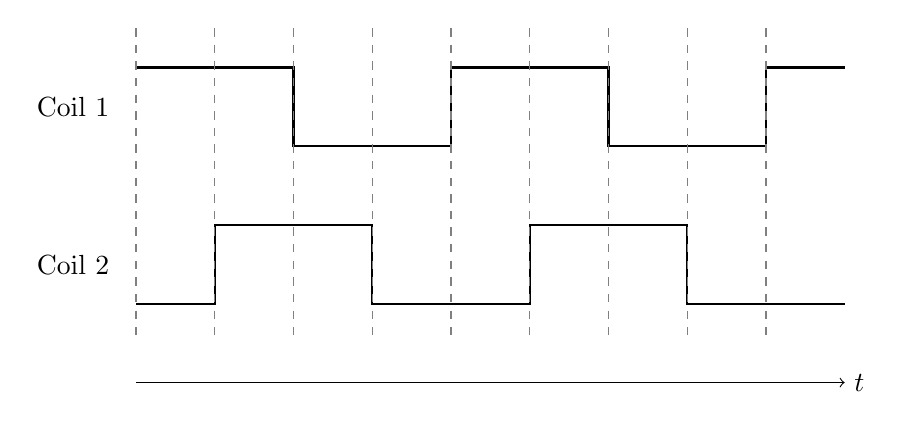
\begin{tikzpicture}[xscale=1.0, yscale=1.0]
        
        % drawing parameters
        \def\T{4} % period length
        \def\A{1} % amplitude
        \def\shift{1} % 90-degree phase shift (T/4)
    
        % label the waves
        \node at (-0.8,0.5) {Coil 1};
        \node at (-0.8,-1.5) {Coil 2};
    
        % first signal
        \draw[thick] 
            (0,\A)
            -- (\T/2,\A) -- (\T/2,0)
            -- (\T,0) -- (\T,\A)
            -- (3*\T/2,\A) -- (3*\T/2,0)
            -- (2*\T,0) -- (2*\T,\A)
            -- (\shift+2*\T,\A);
    
        % second signal is 90 degrees shifted
        \begin{scope}[yshift=-2cm]
        \draw[thick]
            (0,0) -- (\shift,0) -- (\shift,\A)
            -- (\shift+\T/2,\A) -- (\shift+\T/2,0)
            -- (\shift+\T,0) -- (\shift+\T,\A)
            -- (\shift+3*\T/2,\A) -- (\shift+3*\T/2,0)
            -- (\shift+2*\T,0);
        \end{scope}
    
        % x axis
        \draw[->] (0,-3) -- (\shift+2*\T,-3) node[right]{$t$};

        % dashed lines
        \foreach \x in {0,1,2,3,4,5,6,7,8} {
            \draw[dashed, gray] (\x,1.5) -- (\x,-2.5);
        }
        
    \end{tikzpicture}

    \caption{Illustration of the 4 states in the FSM.}
    \label{fig:two-control-signals}
\end{figure}

In practice, the FSM can be implemented by clocking a 74LS163 counter chip and using the bits Q0 and Q1 as outputs, which will allow the counter to go from 0b00 to 0b11 before resetting. To reset the counter, we can detect when Q0 and Q1 are both logic high and send that signal to the reset pin, which is easily achieved with a NAND gate.

We realize that to get the two control signals we need for the two coils, we can simply use Q1 and (Q0 XOR Q1) as the two signals. Further, it can be shown that the stepping frequency of the stepper motor will also be equal to the clock frequency, which is convenient for producing particular musical notes with the motor. A schematic of the counter circuitry is shown in Fig. \ref{fig:fsm-counter-circuit}.

\begin{figure}[h]
    \centering
    \includegraphics[width=1\linewidth]{images/FSMCounter.png}
    \caption{Finite state machine counter.}
    \label{fig:fsm-counter-circuit}
\end{figure}

The current control signals are only enough to turn on one polarity of voltage for each coil in an H-bridge. To be able to turn on voltage in the other direction, we also need the inverses of both signals. To prevent shoot-through in the H-bridges, delay circuits (Fig. \ref{fig:delay-circuit}) are constructed to provide approximately 1 \unit{\micro\second} of delay between turning off one direction and turning on the other. It should be noted that since the audible frequencies have periods much longer than 1 \unit{\micro\second}, this delay has negligible effect on the stepper motion or the sound produced.

\begin{figure}[h]
    \centering
    \includegraphics[width=1\linewidth]{images/delayCircuit.png}
    \caption{Delay circuit.}
    \label{fig:delay-circuit}
\end{figure}

To supply the clock signal to the 74LS163 (the PWM net in Fig. \ref{fig:fsm-counter-circuit}), any TTL square wave could be used, including that from an Arduino for pre-programmed songs. For the purposes of the project, a Schmitt trigger oscillator was made, with buttons connecting a 150 \unit{\nano\farad} capacitor to different resistors to produce oscillations at frequencies corresponding to different musical notes. 

\subsection{Results}

Fig. \ref{fig:h-bridge-control-sigs} shows the control signals for the gate drivers of the two H-bridges. As we can see, the finite state machine circuit is able to create four control waveforms for turning on each "diagonal" on the two H-bridges.

Fig. \ref{fig:h-bridge-out} depicts the voltage at two opposite nodes at the output of the H-bridge (yellow and green), as well as the voltage across the H-bridge (pink) when the input voltage to the H-bridge is 12 volts. Meanwhile, while operating a motor on the output, the waveforms are somewhat less clean due to motor back EMF but overall still of good quality, as shown in Fig. \ref{fig:h-bridge-motor-out}. Thus, we conclude that the FSM motor driver is a success.

\begin{figure}[h]
    \centering
    \includegraphics[width=0.75\linewidth]{four_control_signals.png}
    \caption{Control signals for H-bridges.}
    \label{fig:h-bridge-control-sigs}
\end{figure}

\begin{figure}[h]
    \centering
    \includegraphics[width=0.75\linewidth]{h-bridge-output.png}
    \caption{Voltage across one H-bridge.}
    \label{fig:h-bridge-out}
\end{figure}

\begin{figure}[h]
    \centering
    \includegraphics[width=0.75\linewidth]{h-bridge-output-with-motor.png}
    \caption{Voltage across H-bridge with a motor running.}
    \label{fig:h-bridge-motor-out}
\end{figure}

\section{Feed-forward Boost Converter}
As an additional design challenge, it was decided that the whole system should run off of battery-level voltage (6 volts). To produce the higher voltage that is required to power the stepper, a boost converter was designed to step 6 volts up to 15 volts.

\subsection{Design}
Some design specifications for operation of the boost converter were laid out, including:
\begin{enumerate}
    \item Switching frequency of 30 \unit{\kilo\hertz}.
    \item Output voltage at 15 volts for any input voltage $<15$ volts.
    \item Inductor operating in continuous conduction mode (CCM) for output current as low as 0.4 amps.
    \item Output voltage ripple no more than 10\% (1.5 volts).
\end{enumerate}

Ideally, a feedback loop would be designed to ensure that the output voltage is 15 volts regardless of the input voltage or loading conditions. However, it was determined that implementing current-mode boost converter control would be too complex to create in the allotted time, so instead, a feed-forward system was designed to compute the duty cycle required for the boost converter to step up any input voltage to 15 volts.

To do this, we start with the boost converter gain equation (assuming CCM), which is $$\frac{v_\text{out}}{v_\text{in}} = \frac{1}{1-D}.$$ Rearranging, we find that $D=1-\frac{v_\text{in}}{v_\text{out}}=1-\frac{v_\text{in}}{15}.$ This means that we could find $D$ as a voltage using some straightforward analog arithmetic: a voltage divider can perform the division, and an op amp subtractor can take the difference from 1 volt. However, since $0<D<1$, the op amp would be operating close to the supply rail, which may cause errors in the computation. So instead, we can scale everything by a factor of 5 to avoid being near the rail. This gives $$5D=5-\frac{v_\text{in}}{3}.$$ The circuit that performs this computation is shown in Fig. \ref{fig:calc-duty-cycle}.

\begin{figure}[h]
    \centering
    \includegraphics[width=1\linewidth]{calculate-duty-cycle.png}
    \caption{Duty cycle calculation.}
    \label{fig:calc-duty-cycle}
\end{figure}

To convert the voltage $5D$ into some kind of duty cycle $D$, we can use it as a fixed reference and compare it to some triangle wave. If the reference is a fraction $D$ of the way up the triangle, then using the fixed reference and the triangle wave as the noninverting and inverting inputs of a comparator would produce a square wave with duty cycle $D$. To create an approximate triangle wave, we can use a 555 timer as shown in Fig. \ref{fig:triangle-gen}. The 555 timer oscillates between voltages of $V_{CC}/3$ and $2V_{CC}/3$. If we supply $V_{CC}=5$ volts, then we need our reference to be a fraction $D$ of the way between $1.67$ volts and $3.33$ volts. This would be $1.67 + 5D/3$ volts. To compute this value, the buffers and summer depicted in Fig. \ref{fig:buff-summ} are used. Finally, this computed reference and the trinagle wave from the 555 timer are compared using a comparator to create the control signal for the boost converter, as shown in Fig. \ref{fig:comp}.

\begin{figure}[h]
    \centering
    \includegraphics[width=1\linewidth]{triangle-gen.png}
    \caption{555 timer as triangle wave generator.}
    \label{fig:triangle-gen}
\end{figure}

\begin{figure}[h]
    \centering
    \includegraphics[width=1\linewidth]{buffers-summers.png}
    \caption{Buffers and summer.}
    \label{fig:buff-summ}
\end{figure}

\begin{figure}[h]
    \centering
    \includegraphics[width=0.75\linewidth]{comp.png}
    \caption{Comparator.}
    \label{fig:comp}
\end{figure}

Assuming that the input voltage will always be around 6 volts, then the condition for maintaining CCM in the inductor is $$L>\frac{V_\text{in}(1-D)DT}{2I_\text{load}}$$ which is around 60 \unit{\micro\henry}. For additional insurance of CCM, I chose $L=90$ \unit{\micro\henry} to account for varying duty cycle that may occur due to some variance in the input voltage. This requires 30 turns of wire around a T106-26 micrometals iron powder inductor core.

For the voltage ripple condition, we require $$C\ge \frac{i_\text{out}DT}{\Delta v}.$$ I used a 220 \unit{\micro\farad} electrolytic capacitor in parallel with two 1 \unit{\micro\farad} ceramic capacitors to limit the voltage ripple.

The gate driver for the switching MOSFET in the boost converter is an IR2125, which requires a supply voltage of at least 12 volts to function consistently. This means that we could power the IR2125 with the boost converter output, but only if we first get the boost converter to produce that output without the MOSFET. To initiate this, a self-start circuit was also designed. This circuit pulses current into the inductor when the output voltage is less than 12 volts, forcibly charging the output capacitor until the output voltage is 12 volts. The circuit is shown in Fig. \ref{fig:self-start}.

\begin{figure}[h]
    \centering
    \includegraphics[width=1\linewidth]{self-start.png}
    \caption{Self-start circuit.}
    \label{fig:self-start}
\end{figure}

\subsection{Results}

Figs. \ref{fig:boost-6V-input}-\ref{fig:boost-10V-input} depict the control signal duty cycle and the output waveform for the boost converter when the input voltage is 6, 7.5, and 10 volts. We can see that the duty cycle computation is reasonably close to the correct values that would produce 15 volts on the output, but it is not perfect. Additionally, we can see that the voltage ripple is consistently around 1.2 volts.

\begin{figure}[h]
    \centering
    \includegraphics[width=1\linewidth]{boost-6V-inpt.png}
    \caption{Boost converter output with 6V input.}
    \label{fig:boost-6V-input}
\end{figure}

\begin{figure}[h]
        \centering
        \includegraphics[width=1\linewidth]{boost-7V5-input.png}
        \caption{Boost converter output with 7.5V input.}
\end{figure}
        
\begin{figure}[h]
    \centering
    \includegraphics[width=1\linewidth]{boost-10V-input.png}
    \caption{Boost converter output with 10V input.}
    \label{fig:boost-10V-input}
\end{figure}

\section{Conclusion}

A photo of the whole setup put together is shown in Fig. \ref{fig:hardware}. When using the boost converter to also power the motor driver and motor, the output voltage drops to around 12 volts. Because of this the self-start circuit switches on and off repeatedly, which leads to poor efficiency. When the motor was not running, the DC power supply that was used to supply 6 volts showed that 0.6 amps of current were being drawn. When the motor was running, the DC power supply showed that 1.3 amps were being drawn. This is an efficiency of a measly 48\%. Some solutions for fixing this could be to implement a chopper on the output to limit the amount of current being drawn as well as ensure that the output voltage does not drop so low that the self-start circuit has to turn back on.

\begin{figure}[h]
    \centering
    \includegraphics[width=1\linewidth]{hardware.jpg}
    \caption{Everything put together.}
    \label{fig:hardware}
\end{figure}

Despite the poor efficiency, the motor driver did work as intended, and I was able to play "Mary Had a Little Lamb" on the stepper motor. Additional improvements to pursue in the future would be to lay out the whole system on a PCB to reduce wiring problems, to find ways to improve the efficiency of the circuit, to add over-current, over-voltage, and reverse voltage polarity protection, and to integrate multiple motors together to play the several different parts of a song.


\end{document}
